\chapter{Prevalence modelling and regression methods}

\textcite[p. 311]{fisher1922mathematical} stated that the objective of
statistics is to reduce the data since its volume is impossible 
to comprehend by the researchers. In that sense, few parameters should represent the whole phenomenon catching the most relevant information. 
Years later, Newman studied the theory of modelling which can be divided 
in three aspects \cite[p. 161]{lehmann2012model}: 

\begin{alineas}
  \item models of complex phenomena are created by putting together 
  simple building elements that the researcher is familiar with and can 
  handle; 
  \item there are two types of models: the \textit{explanatory models}, 
  which will be focused on this work, and the \textit{interpolatory formulae}. 
  \item An explanatory theory necessitates a thorough understanding of the scientific context of the problem. In this regard, we investigated questions involving Respondent-driven sampling and prevalence estimation as introduced in Chapter \ref{ch:theoretical-background}. 
\end{alineas}

In this chapter, we develop models that enclose these ideas building each 
block separately. For a Bayesian modelling, we assume that each parameter
of the model has a probability distribution that incorporates the 
researcher's uncertainty about it. For each individual, we observe $k$ 
covariates that are possible risk factors represented by the vector 
$\x_i \in \R^{k}$ of the $i^{th}$ individual. We denote $\theta_i$ the 
probability of the $i$-th individual have been exposed to the disease
that depends on the prevalence $\theta$ and $\x_i$. We also consider the
dependence of sampling from RDS as a spatial random effect. The probability of
positive test in the $i^{th}$ individual is denoted by $p_i$.  

Another important feature of the model is that sensitivity and 
specificity have the same distribution for all individuals and 
it only depends on the test used to diagnose. This is an assumption 
that must be analysed for each particular case. For instance, COVID-19 
Sofia test has different sensibility and specificity for symptomatic and 
asymptomatic individuals \cite[Table 1][p. 3]{mitchell2021performance}.  

From above, we develop three different models: the first considers perfect 
tests, that is, $\gamma_s = \gamma_e = 1$ and no spatial random effect; 
the second considers imperfect tests, regarding $\gamma_s$ and $\gamma_e$, 
but ignoring the RDS structure; and the third one has imperfect tests and 
RDS structure. \improve{Some considerations are made to improve the model's
limitations.}

The implementation of the following models were in the statistical computation
platform Stan \cite{carpenter2017stan} within Python Interface PyStan
\cite{pystan} which uses an implementation for HMC algorithm. All the codes
are written in \autoref{appendix:stan-codes}.

\section{Perfect tests}

The first model supposes the samples are independent and the test is perfect,
which means that $\theta_i = p_i$ for all $i$. Therefore it only considers the risk factors $\x_i$. 

\begin{equation}
  \label{model:perfect-tests}
  \begin{aligned}
    Y_i \mid \theta_i &\sim \bern(\theta_i), \\
    g(\theta_i) &= g(\theta) + \x_i^T\beta, 
  \end{aligned}  
\end{equation}
where $g(\cdot)$ is the $\logit$ function.
The parameter $\beta \in \R^{k}$ is the risk effects. For Bayesian inference, priors on
$\beta$ and $\theta$ must be included. We use $\beta ~ \sim \N(\mu_{\beta}, \Sigma_{\beta})$
and $\theta \sim \betadist(a^{p}, b^p)$, where the vector $\mu_{\beta}
\in \R^{k}$, the symmetric positive-definite matrix $\Sigma_{\beta} \in
\R^{k\times k}$, and the positive real values $a^p, b^p \in \R_{>0}$ are fixed
hyperparameters. Inferences about $\beta$ and $\theta$ are based on the
posterior distribution. Keeping the notation of
Section \ref{sec:glm}, we denote $\boldsymbol{X}$ the covariate matrix. 

\begin{remark}[Interpretation of prevalence]
  \label{remark:interpretation-prevalence}
  According to the model formulation, if the risk factors are zero, i.e $\x_i
  = 0$, the probability of the $i$-th individual having been exposed is the prevalence $\theta$, which means that in
a population with no risk effects, the probability of a person having the
disease is exactly the proportion in this population. 
\end{remark}

\subsection{Identifiability}
\label{sec:perfect-test-identifiability}

A formal definition for identifiability regards the likelihood function \cite[p.
3459]{xie2006measures}:

\begin{definition}
  Let $\mathcal{P} = \{P_{\theta} : \theta \in \Theta\}$ be
  the family of probability distributions for $\mathcal{Y}$. This model is
  {\em identifiable} if for any $\theta', \theta'' \in
  \Theta$, 
  $$\forall y \in \mathcal{Y}, P_{\theta'}(Y = y) =
  P_{\theta''}(Y = y) \implies
  \theta' = \theta''.$$ 
\end{definition} 

The family distribution from model \eqref{model:perfect-tests} is the logistic
regression parametrized by $(\theta, \beta)$ and conditioned on
observing the regressor $\boldsymbol{X}$, with $\mathcal{Y} = \{0,1\}^n$. Defining $\beta_0 =
g(\theta)$, we may rewrite it as 
$$Y_i \mid \tilde{\beta}, \tilde{\x}_i \sim \bern(g^{-1}(\tilde{\x}_i^T\tilde{\beta})),$$
such that $\tilde{\beta}$ concatenate $\beta_0$ and $\beta$, and $\tilde{\x}_i$
concatenate $1$ and $\x_i$. \textcite[p. 7]{kuchenhoff1995identification}
gives a formal proof for the identifiability of this representation.

In the Bayesian paradigm, inferences are based on the posterior distribution.
Therefore, identifiability should consider the prior distribution.
\textcite[p. 46]{lindley1972bayesian}  argued that proper priors are
sufficient to handle
identifiability problems in the Bayesian perspective, which means that a
well-defined posterior probability distribution is enough for parameter
identification. A formal definition for {\em Bayesian identifiability} is the
following: if $p(\theta \mid \beta, y, \boldsymbol{X}) = p(\theta \mid
\beta)$, the data $y$ is uninformative for $\theta$ when $\beta$ is known. 
The definition is analogous if $\beta$ and $\theta$ change places. However,
\textcite[p. 248]{gelfand1999identifiability} proved that this definition is equivalent to
likelihood identifiability. 

Despite the identifiability of the model, it may be hard to sample from
the posterior distribution depending on the value of $\x$. As an example, 
consider the following experiment: 

\begin{enumerate}[label=(\roman*)]
  \item generate $500$ covariates $X_i \sim \N(15, 1)$;
  \item let $\beta = 0.1$, $\theta = 0.1$, and $\theta_i = g^{-1}(g(\theta) +
  X_i\beta)$ for $1 \le i \le 500$;
  \item for each $i$, sample $Y_i \sim \bern(\theta_i)$;
  \item let $a^p = 1$, $b^p = 1$, $\mu_{\beta} = 0$, and $\Sigma_{\beta} = 1$
  the hyperparameters for the prior distributions (weakly informative);
  \item make 1000 warm-up and 1000 sampling iterations using Stan given the
  data $(Y_1, X_1), \dots, (Y_n, X_n)$.  
  \item make 2000 warm-up and 2000 sampling iterations using Stan given the
  data $(Y_1, X_1), \dots, (Y_n, X_n)$.
\end{enumerate}

The HMC sampler took around 8.39s.
\autoref{fig:result-uncentered-mean} presents the results through the posterior
distribution, the trace plot, and the strong posterior
correlation between $\theta$ and $\beta$. To address this 
problem, subtracting the mean $\bar{x}$ is a default procedure \cite[p.
5]{ogle2020ensuring}. After centering the data around the mean, the HMC
sampler took around 1.39s, and the improved results are shown in
\autoref{fig:result-centred-mean}. 

\begin{figure}
  \centering  
  \caption{\label{fig:result-uncentered-mean}Posterior
  distribution, trace plot, and posterior samples of parameters 
  $\theta$ and $\beta$ from model \eqref{model:perfect-tests} with uncentered covariate.}
  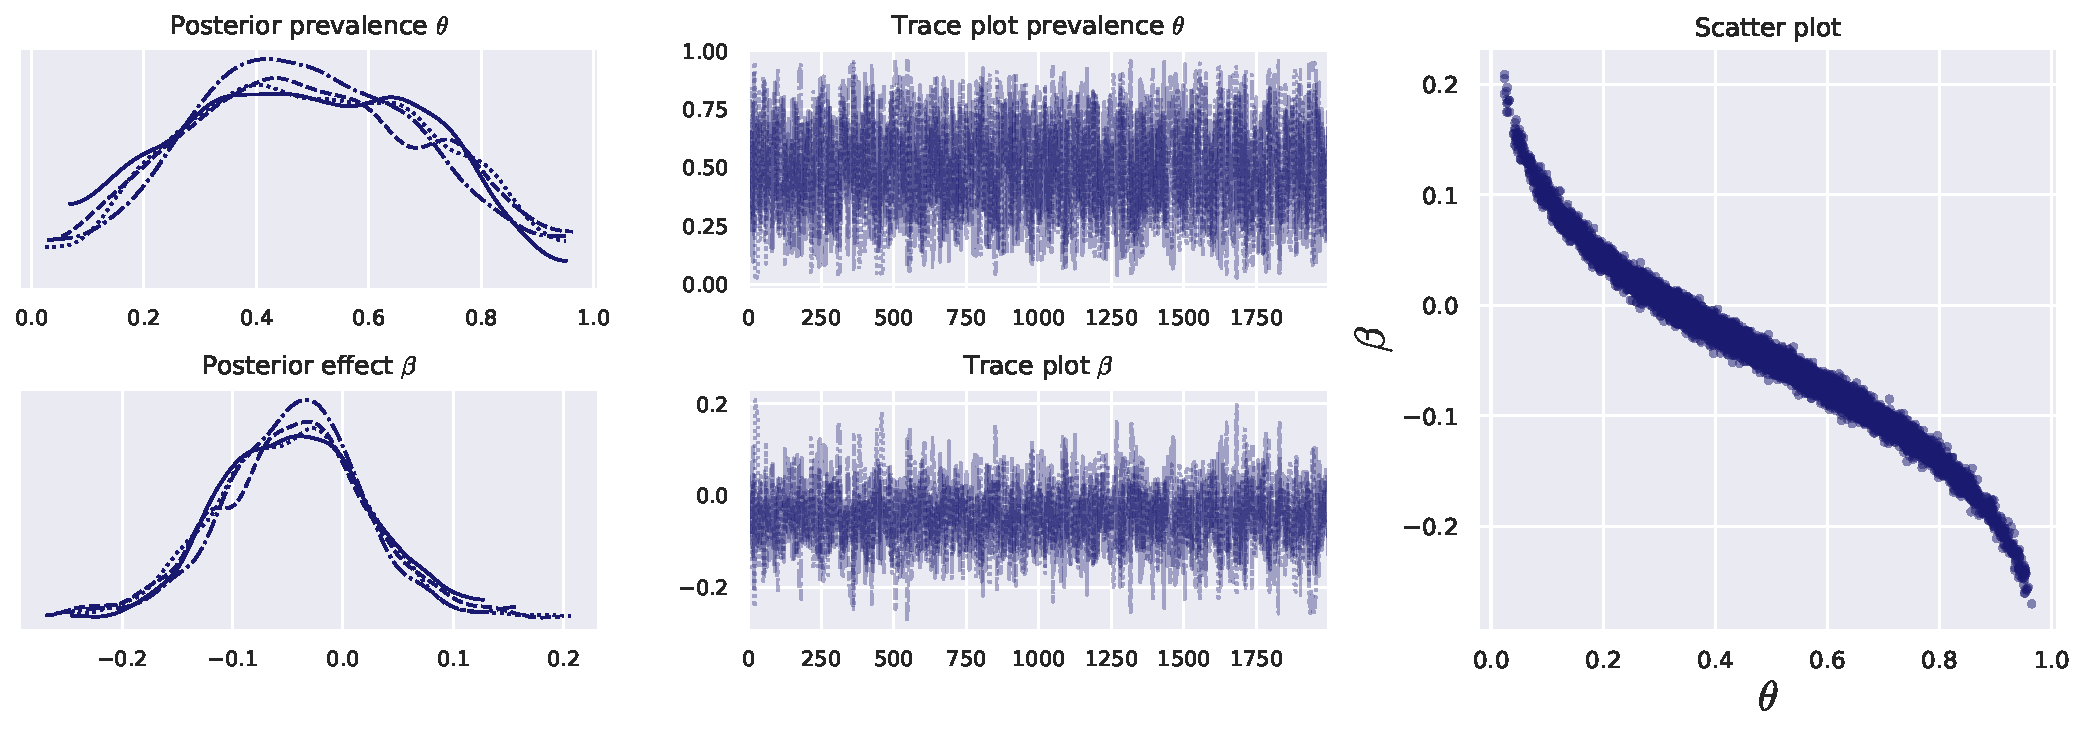
\includegraphics[width=14cm]{identifiability_perfect_tests_unscaled_x.pdf}
  \fonte{Prepared by the author (2021).}
\end{figure} 

\begin{figure}
  \centering  
  \caption{\label{fig:result-centred-mean}Posterior
  distribution, trace plot, and posterior samples of parameters 
  $\theta$ and $\beta$ from model \eqref{model:perfect-tests} with centralized covariate.}
  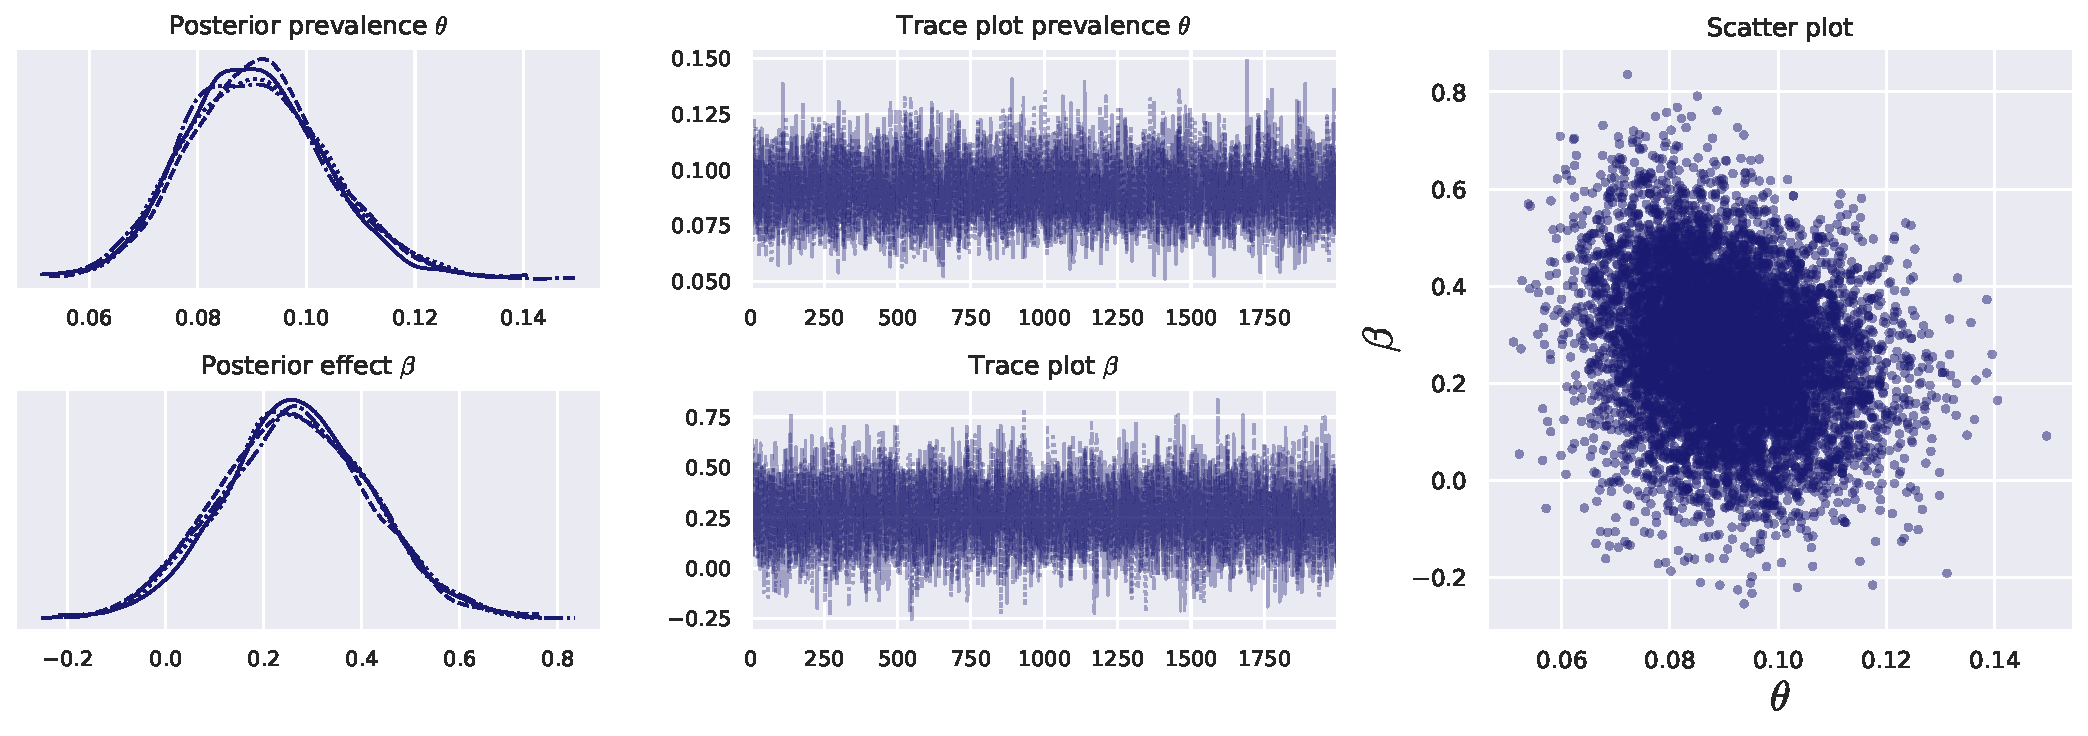
\includegraphics[width=14cm]{identifiability_scaled_x.pdf}
  \fonte{Prepared by the author (2021).}
\end{figure} 

We observe that the interpretation of prevalence from Remark
\ref{remark:interpretation-prevalence} changes from centred and 
uncentered since the meaning of $\x_i = 0$ is different. Along with this
discussion, it is usual to divide the centred variable by its
standard deviation, to put all predictors on a common scale. Discussions about
the problems caused by standardizing are outside the scope of this work. 
\textcite{gelman2008scaling} suggests to divide de continuous variables by 2
times de standard deviation to allow ``the coefficients to be interpreted in
the same way as binary deviation.'' \cite[p. 2867]{gelman2008scaling} Binary
inputs are not standardized since their coefficients are easily interpretable.

Other identifiability problems arising from the input variables are
collinearity and {\em separation} \cite[p. 1360-1361]{gelman2008weakly}. 
The latter occurs if a linear combination of a subset of the predictors gives
a perfect prediction for the binary outcome. For instance, when a linear
combination of the predictors is greater than a threshold if and only if $y =
1$.  

\subsection{Simulated data}

To present a sanity check about the functionality of model
\eqref{model:perfect-tests} and to validate the properties of the estimation
procedure, we simulate fake data from the model and make inferences about the
result. We follow the experiment from Section
\ref{sec:perfect-test-identifiability}.
\autoref{table:experiments-perfect-test} summarizes the experiment
parameters. 

\begin{table}[!ht]
  \centering
  \caption{\label{table:experiments-perfect-test}Experiment settings for the
  simulation of model \eqref{model:perfect-tests}.}
  \begin{tabular}{ccccccc}
  \hline
  Exp & $n$ & $k_{c}$ (normal) & $k_{c}$ (cauchy) & $k_{b}$ & $\beta$ & $\theta$ \\ \hline
  \multicolumn{1}{c}{1} & 100 & 3 & 0 & 2 & {[}-0.1, 2.5, 1.4, -1.8, 0.3{]} & 0.05 \\
  \multicolumn{1}{c}{2} & 100 & 3 & 0 & 2 & {[}-0.1, 2.5, 1.4, -1.8, 0.3{]} & 0.9 \\
  \multicolumn{1}{c}{3} & 100 & 2 & 2 & 1 & {[}-0.1, 2.5, 1.4, -1.8, 0.3{]} & 0.1 \\
  \multicolumn{1}{c}{4} & 5000 & 40 & 5 & 5 & $F$ distribution & 0.1 \\\hline
  \end{tabular}
  \fonte{Prepared by the author (2021). We denote $n$ for number of samples,
  $k_c$ for the number of continuous variables, and $k_b$ for binary variables. Between
  paranthesis, \textit{normal} means that the variables were generated from a
  Multivariate Normal with prespecified parameters, and \textit{cauchy} from a
  Cauchy distribution. $F$ distribution is $\N(\mu = 0, \sigma = 2)$ with
  probability 0.3, and 0 otherwise.}
\end{table}

We primally look at the settings from experiment 1. With a non-informative prior for $\theta$
(Jeffreys prior $\betadist(1/2, 1/2)$) and a weakly informative for $\beta$
(zero mean and covariance matrix four times the identity matrix),
\autoref{fig:result-experiment1-perfect-test} shows the posterior
distributions for the parameters. The prevalence estimate is good despite
Jeffreys' prior. When the distance between the prior and the true value is large, the
inferences seem to be biased. However, this makes sense regarding the model. For
instance, for $\beta_2$, before observing the data, we put 0.7 mass probability
for values lesser than 0.1. The data decreased it to 0.125. This highlights
the importance of a well defined prior distribution. The values for Bulk ESS
was greater than 3000 for all parameters, while Tails ESS were greater that
2200 with 1000 warmup and 1000 sampling iterations, and 4 chains. For all
parameters $\hat{R} = 1$. Trace plots and scatter plots were also good and we
omit here since they do not bring new information for the discussion. 

\begin{figure}[!ht]
  \centering  
  \caption{\label{fig:result-experiment1-perfect-test}Posterior
  distribution for parameters of model \eqref{model:perfect-tests}.}
  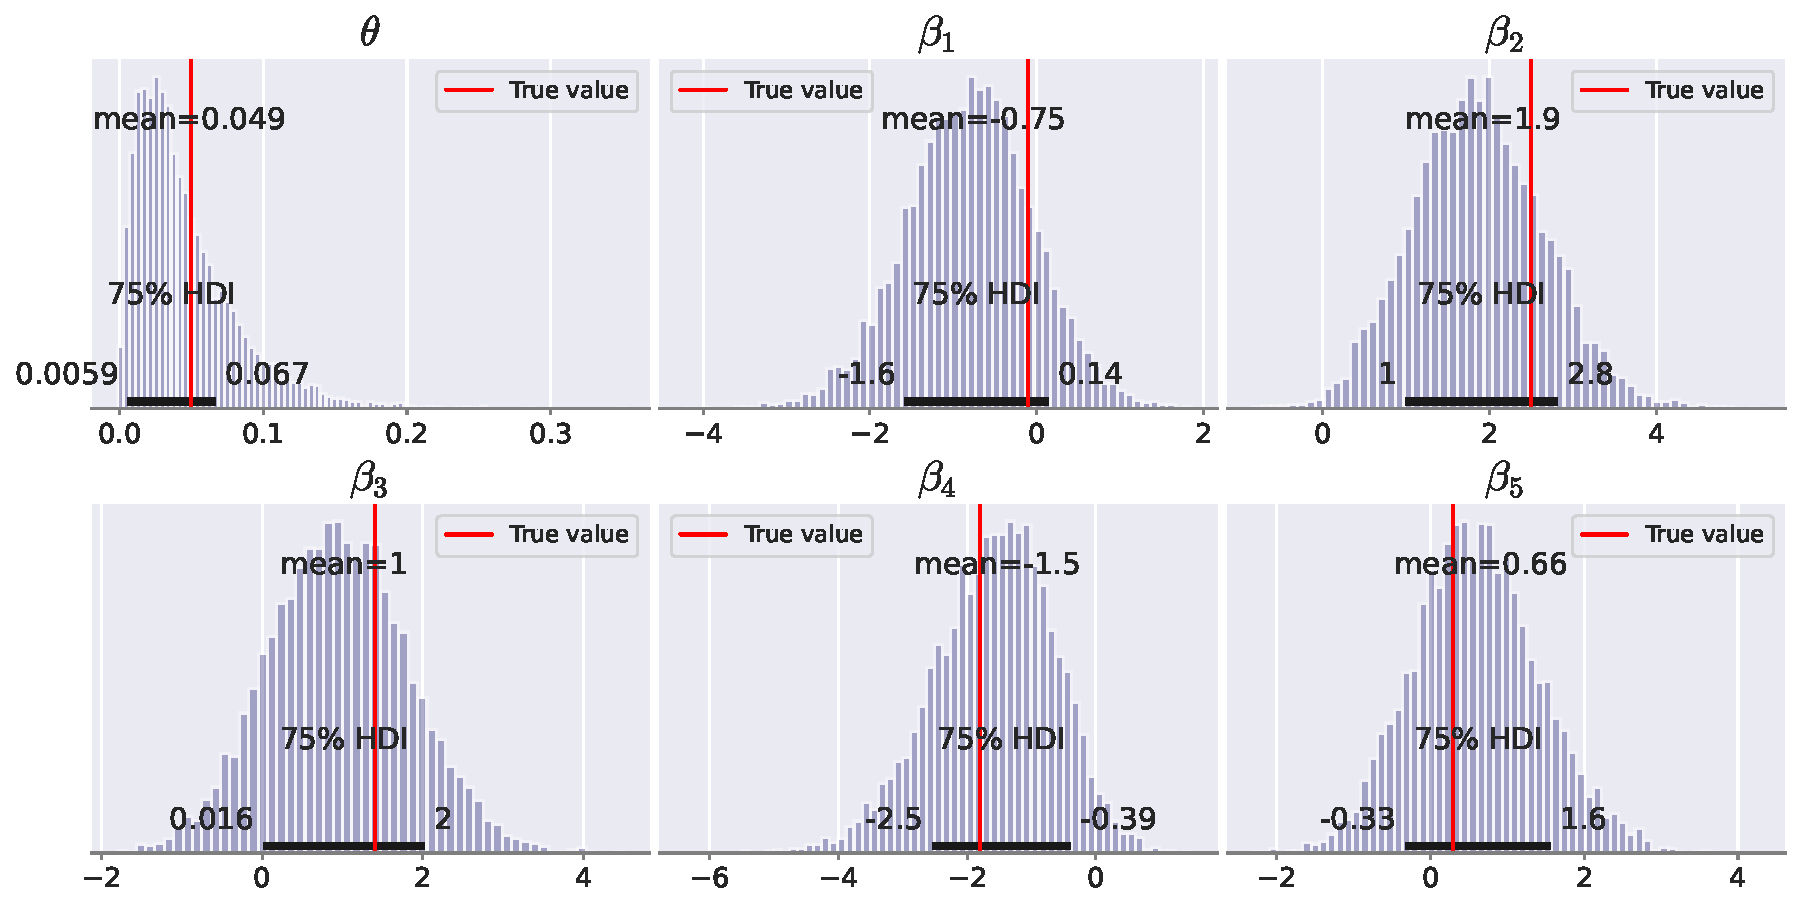
\includegraphics[width=14cm]{posterior_perfect_tests_exp1.pdf}
  \fonte{Prepared by the author (2021).}
\end{figure} 

Although we are performing Bayesian inference, frequentist properties can me
accessed through simulation. After 1000 simulations varying the input data
$Y$, the 75\% credible interval included the true parameters in 75.8\%, 78.8\%,
76.4\%, 77.5\%, 67.3\%, and 72.2\% of the times, respectively for $\theta,
\beta_1, \dots, \beta_5$. Each simulation had 100 samples and weakly
informative priors for $\beta$ and $\theta$.
\autoref{fig:predicted-vs-simulated-perfect-tests} compares the predicted and
simulated probabilities. The green area is delimited by the curves generated
by $2\sqrt{\theta_i(1-\theta_i)/n}$, where $n=500$ is the number of points. 
It was increased to show a larger variety of points. This area is a $\pm 2$
standard-error bounds. 

\begin{figure}[!ht]
  \centering  
  \caption{\label{fig:predicted-vs-simulated-perfect-tests}Comparing predicted
 and simulated probabilities of having the disease from model \eqref{model:perfect-tests}.}
  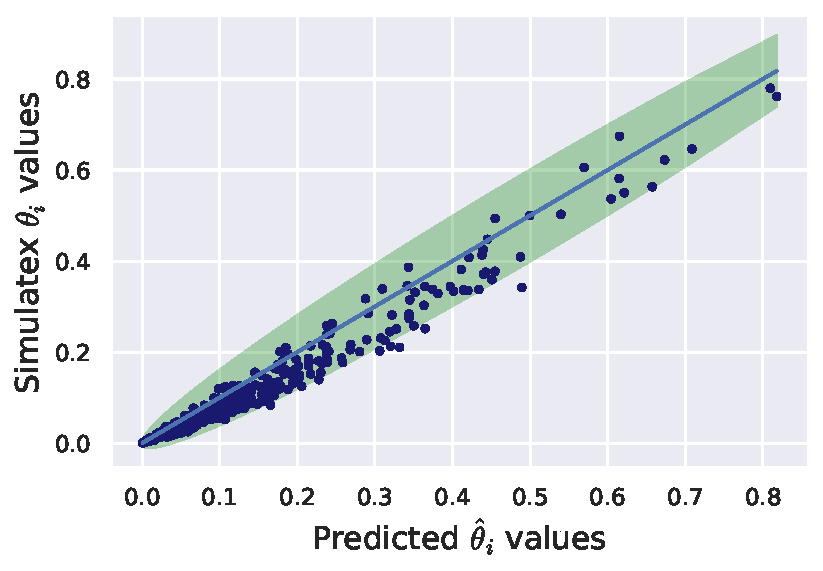
\includegraphics[width=10cm]{predicted-vs-simulated-perfect-tests.pdf}
  \fonte{Prepared by the author (2021).}
\end{figure} 

Experiment 2 is used to see if these properties repeat when the prevalence is
higher. The same regressors were used for the comparison, but the input data
$Y$ were generated with different prevaleces. With prevalence being 0.9, the
estimates were a little high for all coefficients as
\autoref{fig:comparing-diff-prevalence-perfect-tests} presents. This is
related to the fact that the posterior mean underestimated the true value for this
experiment. After increasing the number of samples, the estimates were closer,
as expected. 

\begin{figure}[!ht]
  \centering  
  \caption{\label{fig:comparing-diff-prevalence-perfect-tests}Comparing
  posterior mean and 94\% credibility intervals for $\beta$ in model \eqref{model:perfect-tests} with the same regressors
  $\boldsymbol{X}$ but different prevalences.}
  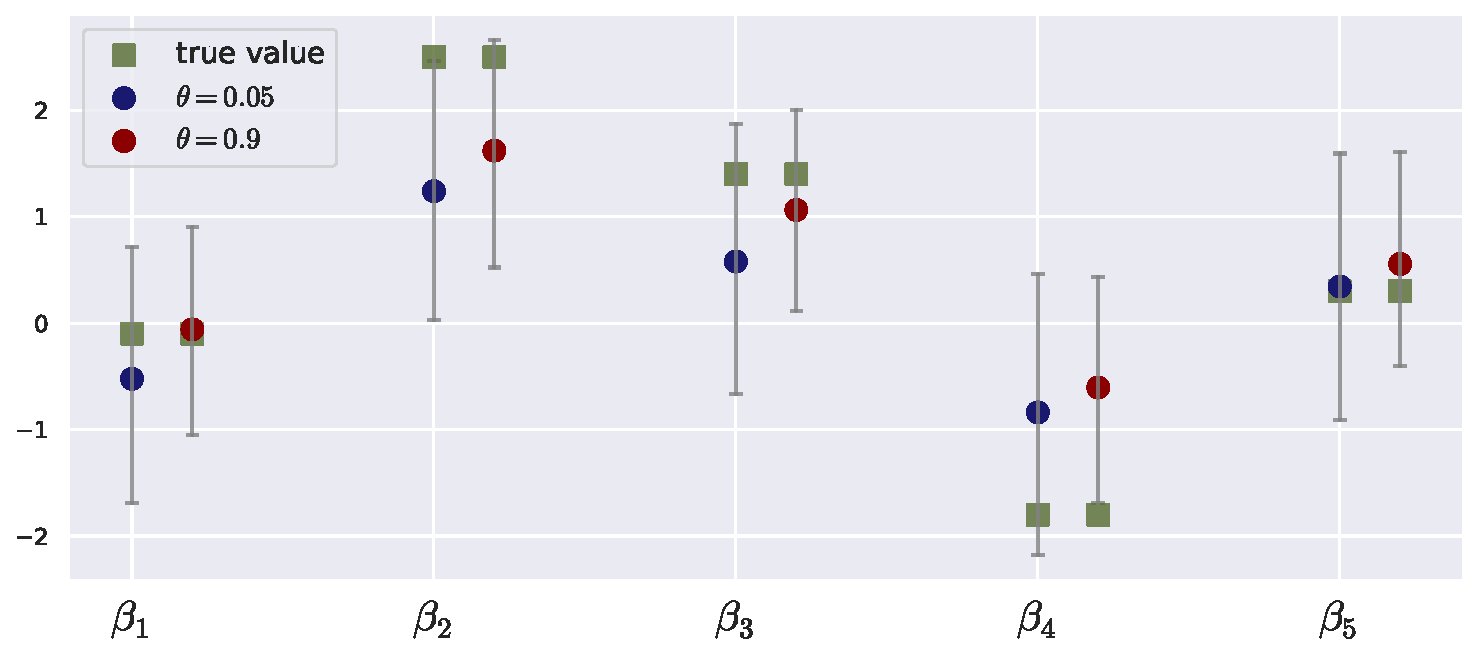
\includegraphics[width=12cm]{comparing-diff-prevalence-perfect-tests.pdf}
  \fonte{Prepared by the author (2021).}
\end{figure} 

The third experiment aims to analyse what happens if some covariates have a
heavier tail. No big difference was noticed despite the existence of some
individuals very different from the others. At last, the fourth experiment
increases the dimensionality to observe the number of effective samples. Each
chain took around 3 minutes, instead of the 3s needed for the previous
experiments. From the 51 parameters, 48 had the true values in the 95\% HDI
credible interval. The Bulk ESS was greater than 4500 for 95\% of the
parameters. \autoref{fig:predicted-vs-simulated-high-dimension-perfect-tests}
presents how the predicted probabilities for each individual behaves in this
case. Here the green area is delimited by the 95\% credible interval. 

\begin{figure}[!hb]
  \centering  
  \caption{\label{fig:predicted-vs-simulated-high-dimension-perfect-tests}
  Comparing predicted and simulated probabilities of having the disease from
  model \eqref{model:perfect-tests} with high dimension.}
  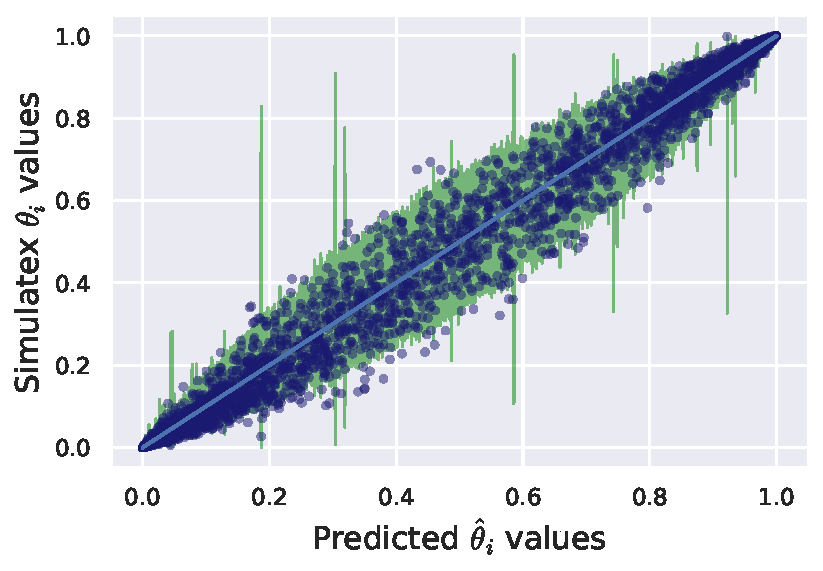
\includegraphics[width=10cm]{predicted-vs-simulated-high-dimension-perfect-tests.pdf}
  \fonte{Prepared by the author (2021).}
\end{figure} 

\section{Sensitivity and specificity}

In this section, we describe a model for estimating the sensitivity and
specificity of a diagnostic test. This model is relevant to analyze and
experiment with different prior specification approaches. Suppose having a
gold standard test and another test, for instance, a simpler, faster, or less
invasive one, which we want to estimate the accuracy by the sensitivity and
specificity. In this scenario,
true positive (negative) individuals are those who tested positive (negative) by
the gold standard. Therefore, in a population with $n_{\gamma_s}$ true
positives and  $n_{\gamma_e}$ true negatives, we denote 
\begin{gather*}
  y_{\mathrm{pos}} \mid \gamma_s \sim \operatorname{Binomial}(n_{\gamma_s}, \gamma_s),\ \\
  y_{\mathrm{neg}} \mid \gamma_e \sim \operatorname{Binomial}(n_{\gamma_e}, \gamma_e), 
\end{gather*}
such that $y_{\mathrm{neg}}$ are negative tests on known negative 
subjects and $y_{\mathrm{pos}}$ are positive tests on
known positive. In the Two-by-two formulation from \autoref{table:two-by-two},
we have

\begin{quadro}[!ht]
  \centering
  \caption{\label{table:two-by-two-data}Two-by-two table with the model specification.}
  \begin{tabular}{c|c|c|c|}
  \cline{2-4}
                                               & $Y = 0$ & $Y = 1$ & Total\\ \hline
  \multicolumn{1}{|c|}{$Y^{\mathrm{true}}= 0$} & $y_{\mathrm{neg}}$  & $n_{\gamma_e} - y_{\mathrm{neg}}$ & $n_{\gamma_e}$ \\ \hline
  \multicolumn{1}{|c|}{$Y^{\mathrm{true}}= 1$} & $n_{\gamma_s} -
  y_{\mathrm{pos}}$    & $y_{\mathrm{pos}}$  & $n_{\gamma_s}$  \\ \hline
  \multicolumn{1}{|c|}{Total} & $n_{\gamma_s} + y_{\mathrm{neg}} -
  y_{\mathrm{pos}}$ & $n_{\gamma_e} + y_{\mathrm{pos}} - y_{\mathrm{neg}}$ &
  $n_{\gamma_s} + n_{\gamma_e}$ \\\hline
  \end{tabular}
  \fonte{Prepared by author (2021).}
\end{quadro}

In Bayesian analysis, we have to define a prior distribution with density $\pi$ for the
parameters $(\gamma_e, \gamma_s)$. For this, we consider three different approaches: 

\begin{alineas}
  \item prior distributions are specified independently for each parameter and
  each one has a beta distribution, i.e,  
  $$\pi(\gamma_e, \gamma_s) =
  \pi(\gamma_e)\pi(\gamma_s) \propto \gamma_s^{a_s}(1-
  \gamma_s)^{b_s}\gamma_e^{a_e}(1-\gamma_s)^{b_e},$$
  for $a_s, b_s, a_e,$ and $b_e$ being pre-determined positive real hyperparameters;
  \item bivariate normal distribution in the log odds space, i.e,  
  $$(\logit(\gamma_e), \logit(\gamma_s)) \sim
  \N(\mu_{\gamma}, \Sigma_{\gamma}),$$
  such that the vector $\mu_{\gamma} \in \R^2$ and the covariance matrix
  $\Sigma_{\gamma} \in \R^{2\times 2}$ are pre-determined hyperparameters;
  \item a bivariate beta distribution described in Appendix \ref{appendix:bivariate-beta-distribution}
  with parameters $\alpha_1, \dots, \alpha_4 \in \R_{>0}$.
\end{alineas}

\subsection{Independent beta distribution priors}

If the knowledge of the specificity affects the range of most possible values
of the sensitivity, or vice-versa, there is antecedent information about the
correlation between the parameters. When this is not the case, a possible
independent prior formulation is the usage of $\betadist$ distribution since
it is bounded in the interval $[0,1]$ and it is reasonably flexible in its
shape.  Another good reason for this choice is that the beta distribution forms a conjugate family with the binomial
distribution, that is, if the likelihood has binomial distribution and the
prior has beta distribution, then the posterior has beta distribution.


When considering separated experiments for specificity and
sensitivity, there is
no information about their correlation, which is the case for our model. Then we define the the prior distributions
\begin{gather*}
  \gamma_e \sim \operatorname{Beta}(a_e, b_e), \\
  \gamma_s \sim \operatorname{Beta}(a_s, b_s), \\
  \theta \sim \operatorname{Beta}(a_{\theta}, b_{\theta}).
\end{gather*} 
Using data from \cite{bennett2020estimating} about COVIDPrior information of these quantities lead to a bivariate analysis {cite:t}`guo2017bayesian`. As we have already mentioned, the definitions of *sensitivity* and
*specificity* can be expressed as below: -19 seroprevalence in
Santa Clara:  
\begin{align*}
  y/n &= 50/3330,\\
y_{neg}/n_{\gamma_e} &= 399/401, \\
y_{\mathrm{pos}}/n_{\gamma_s} &= 103/122, 
\end{align*}
we fit the model and obtain the results showed in Figure
\ref{fig:results-posterior-model1}. All the codes were done in {\em Stan} and
{\em PyStan}.

\begin{figure}[!ht]
  \centering
  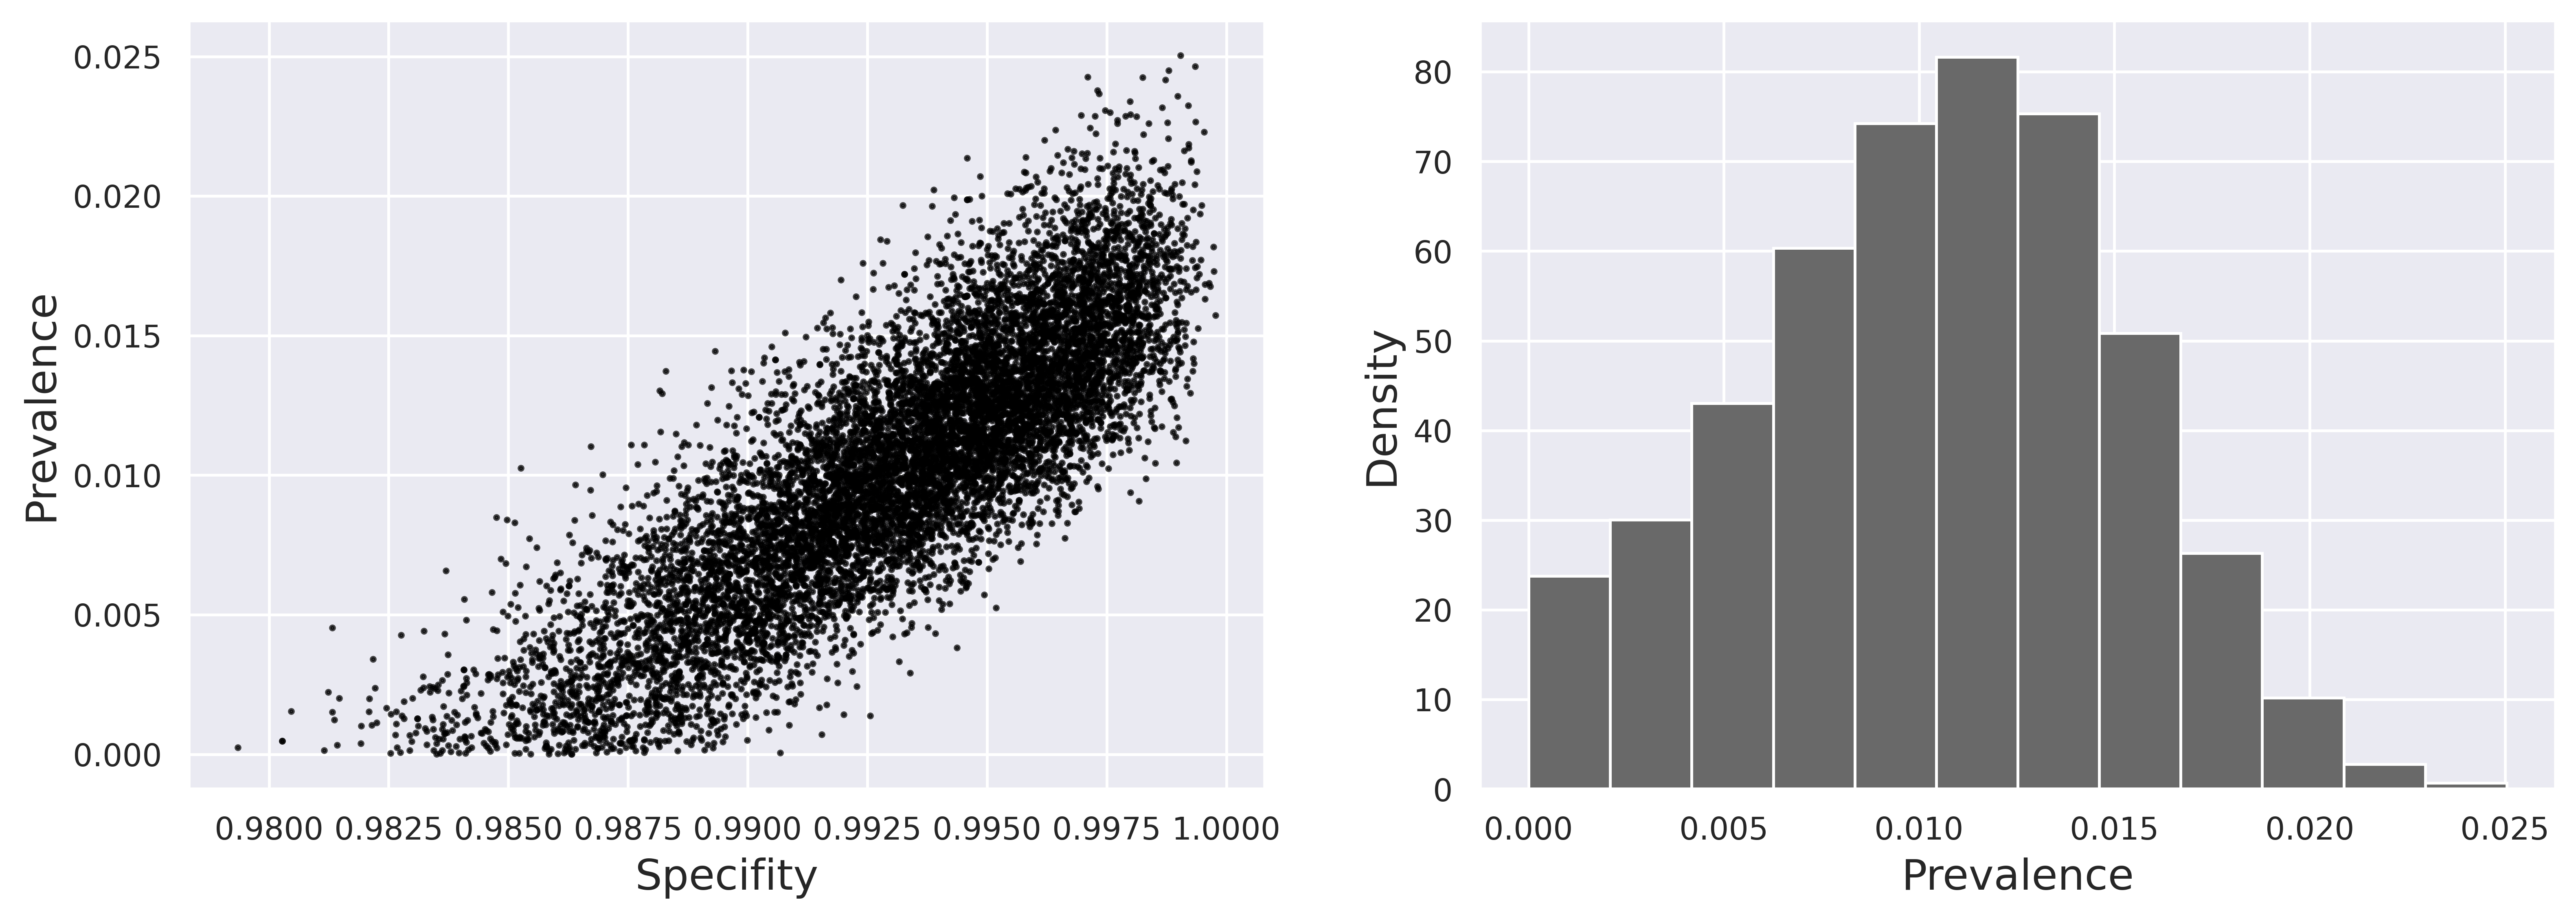
\includegraphics[width=\textwidth]{../../images/model1_gelman_figure_english.png}
  \caption{Scatter plot of posterior simulations of prevalence against
  specificity and histogram of posterior simulations of the prevalence.}
  \label{fig:results-posterior-model1}
\end{figure}

\subsection{Hierarchical partial pooling prior}

Other approach considers more than one study about specificity and
sensitivity. A {\em hierarchical partial pooling} model for these studies
can be done in the following way: 
\begin{gather*}
    \logit(\gamma_s^j) \sim \operatorname{Normal}(\mu_{\gamma_s}, \sigma_{\gamma_s}), \\
    \logit(\gamma_e^j) \sim \operatorname{Normal}(\mu_{\gamma_e}, \sigma_{\gamma_e}), 
\end{gather*}
for $1 \le j \le K$ studies, such that the first study is the considered one.
Partial pooling because the parameters can be sampled from the same
distribution. Hierarchical because the parameters of this distribution have
its one prior distributions. For instance, 
\begin{align*}
    \mu_{\gamma_s} &\sim N(0, 10), \\ 
    \mu_{\gamma_e} &\sim N(0, 10), \\
    \sigma_{\gamma_s} &\sim N^+(0,1), \text{ and } \\
    \sigma_{\gamma_e} &\sim N^+(0,1),
\end{align*}
where $N^+(a,b)$ is the truncated normal distribution in $[0,+\infty)$.

\subsection{Bivariate Beta prior}

Finally, we studied a joint distribution for specificity and sensitivity, a
possible bivariate beta distribution built in \cite{olkin2015constructions}.
This distribution is derived from a Dirichlet distribution of order four. Let $U = (U[1],...,U[4]) \sim \operatorname{Dirichlet}(\boldsymbol{\alpha})$, where
$\boldsymbol{\alpha} \in \mathbb{R}^4_+$. Therefore, defining $X = U[1] +
U[2]$ and $Y = U[1] + U[3]$, we will have that $(X,Y)$ has a well-defined
probability distribution in
$[0,1] \times [0,1]$ such that $X$ and $Y$ have marginally beta distributions,
and they have correlation in all space. Depending on the definition of
$\boldsymbol{\alpha}$, the correlation between the variables range from -1 and
1. Figure \ref{fig:beta-bivariate} shows some examples of this construction. 

\begin{figure}[!ht]
    \centering
    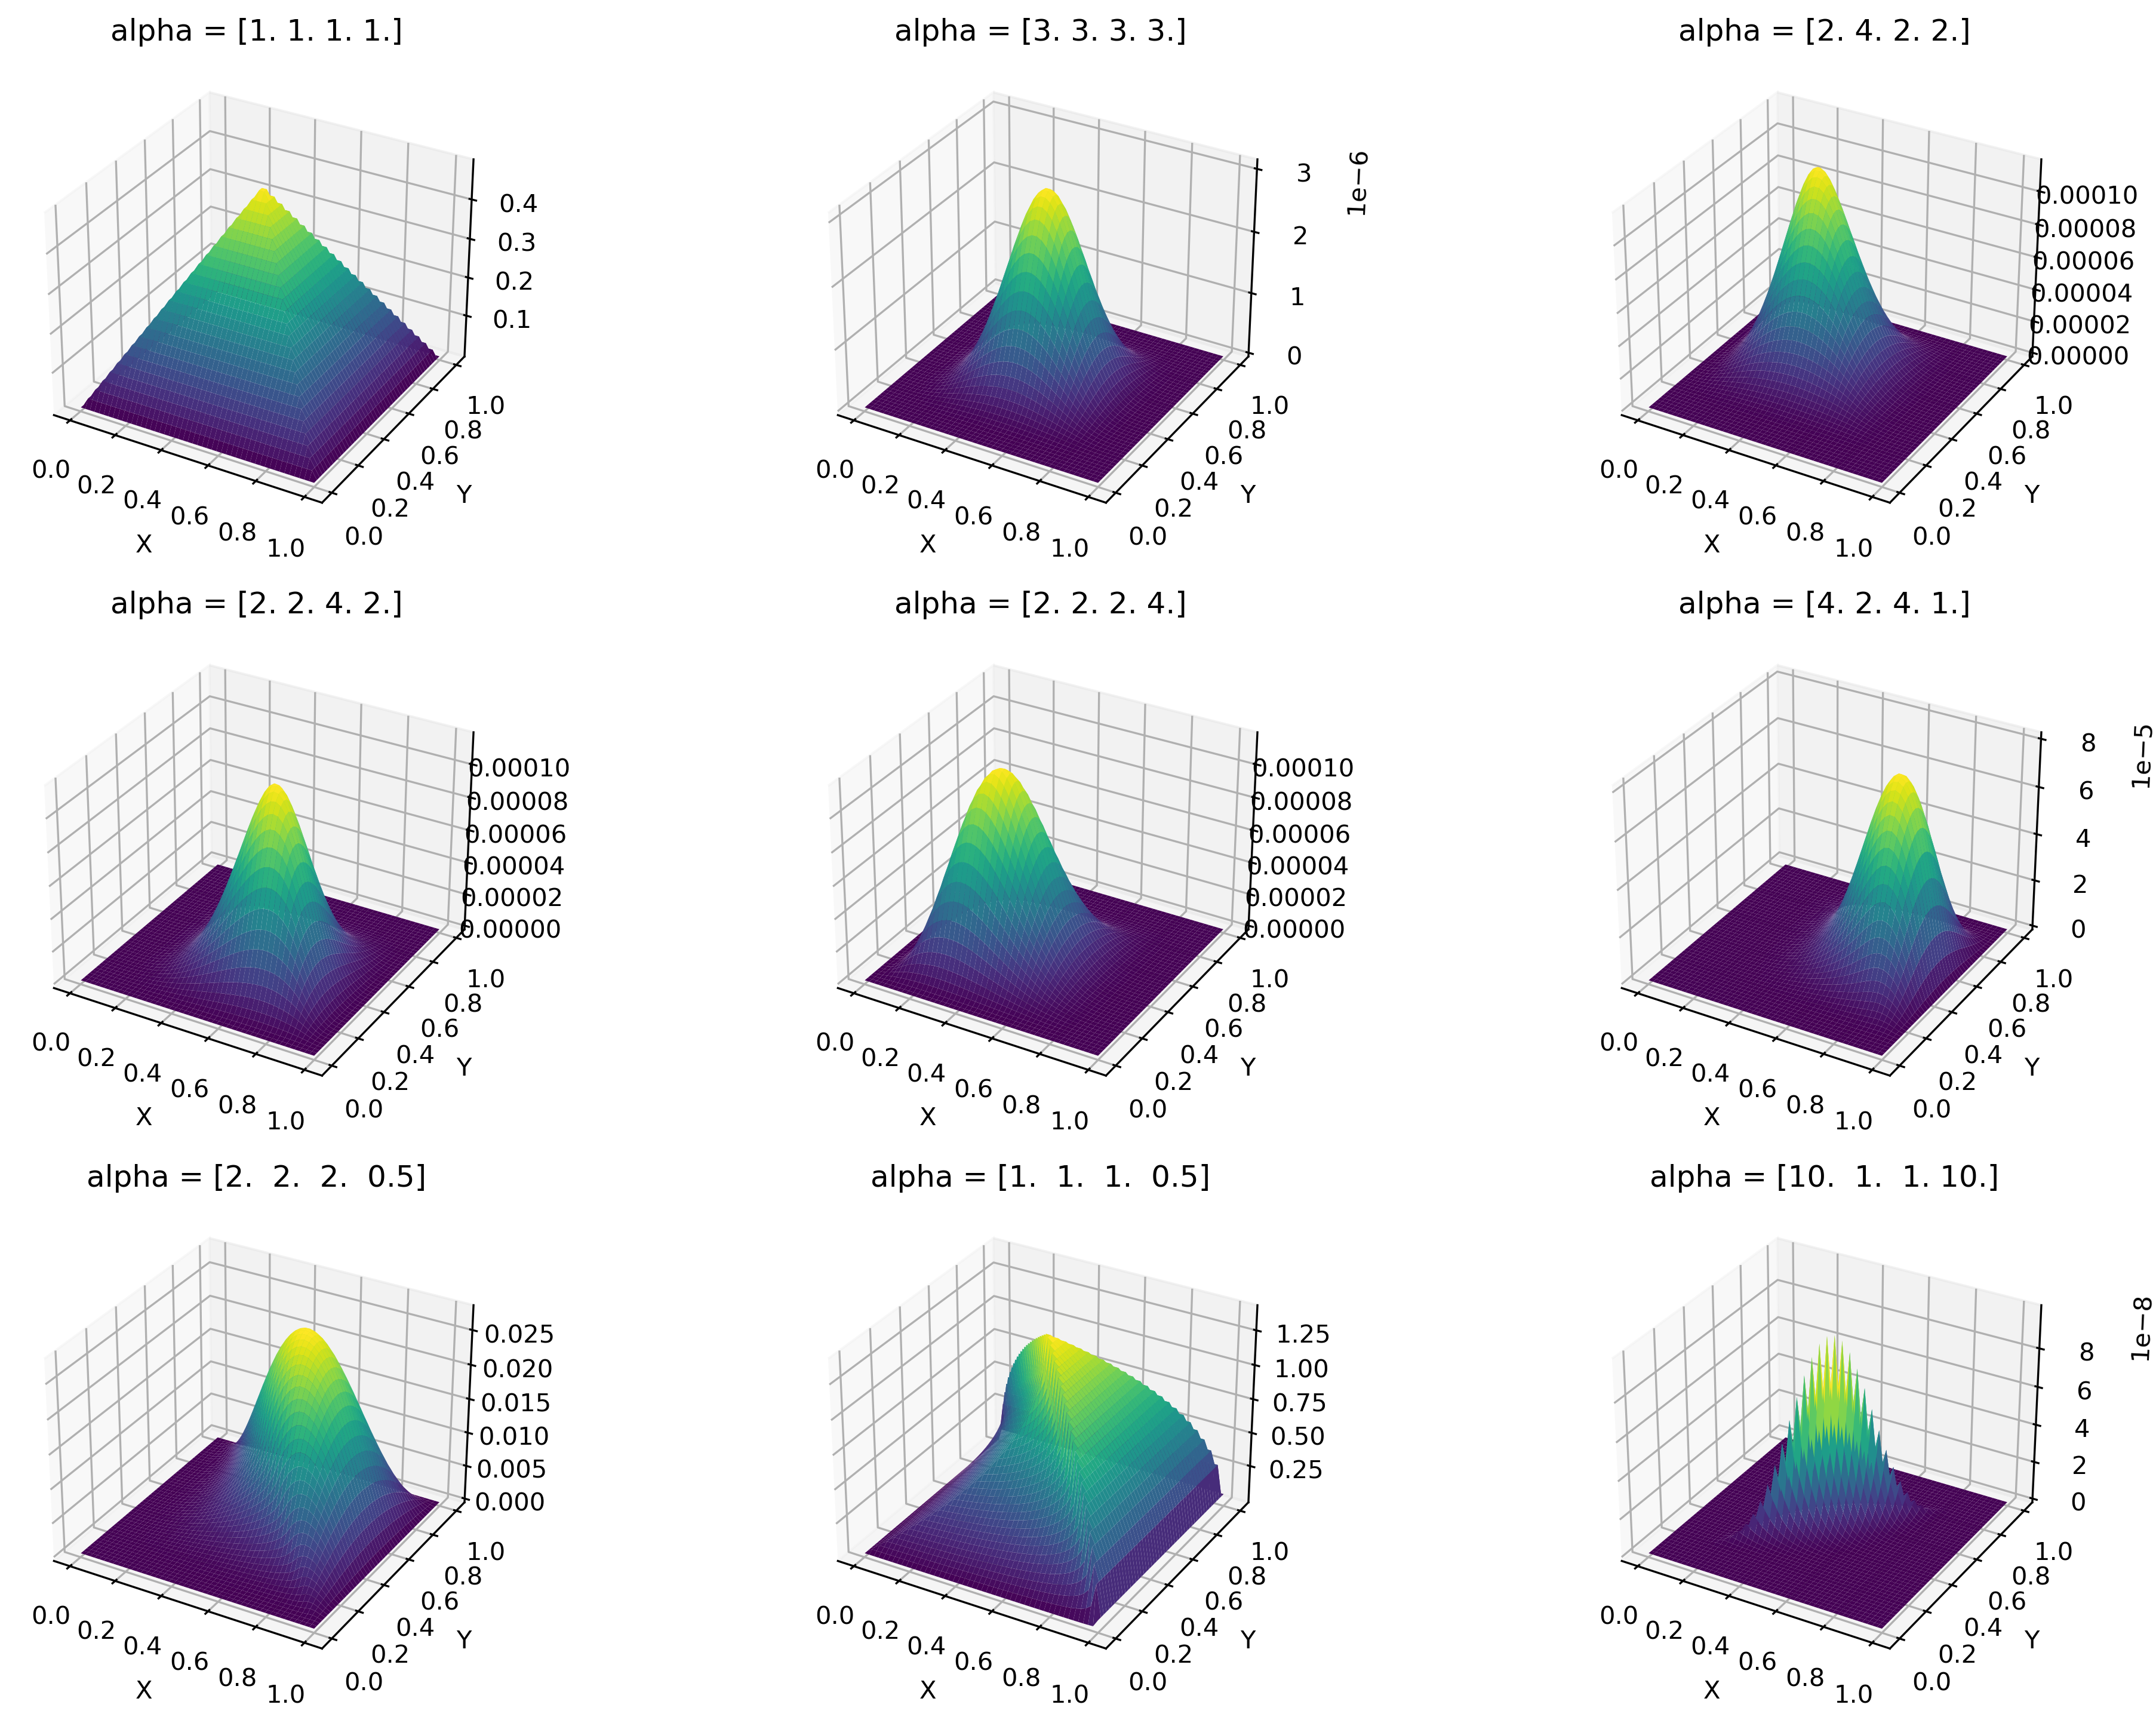
\includegraphics[width=\textwidth]{beta-distributions.png}
    \caption{Different choices of $\alpha$ and the joint distribution of the variables $X$ and $Y$.}
    \label{fig:beta-bivariate}
\end{figure}

In this section, we shall describe how to use the Bivariate Beta (see Appendix
\ref{appendix:bivariate-beta-distribution}) to model the correlation between
specificity and sensitivity.

\section{Imperfect tests}

This model includes the sensitivity and specificity of the diagnostic test. 

\begin{equation}
  \begin{aligned}
    T_i &\sim \bern(p_i) \\
    p_i &= \gamma_s\theta_i + (1-\gamma_e)(1 - \theta_i),  \\
    g(\theta_i) &= g(\theta) + \x_i^T\beta,  \\
    \beta &\sim \N(\mu, \Sigma), \\ 
    \theta &\sim \betadist(a^p, b^p) \\
    \gamma_s &\sim \betadist(a^s, b^s), \\
    \gamma_e &\sim \betadist(a^e, b^e), \\    
  \end{aligned}  
\end{equation}
where $a^p, a^s, a^e, b^p, b^s, b^e \in \R_{++}$ are fixed hyperparameters.
This model does not include prior knowledge about the correlation between
specificity and sensitivity. 

\subsection{Simulated data}

Consider the following model \cite{gelman2020bayesian}:
\begin{gather*}
  y \sim \operatorname{Binomial}(n, p), \\
  p = \theta\gamma_s + (1- \theta)(1-\gamma_e), 
\end{gather*}
such that $y$ is the number of positive tests in a population of size $n$. In
a Bayesian paradigm, a prior $\pi(\theta, \gamma_e, \gamma_s)$ must be
specified. For instance, $\pi(\theta, \gamma_e, \gamma_s) =
\pi(\theta)\pi(\gamma_e, \gamma_s)$ and $\theta \sim
\operatorname{Beta}(\alpha_{\theta}, \beta_{\theta})$, in which
$\alpha_{\theta}$ and $\beta_{\theta}$ are positive hyperparameters. Since the
three parameters $\theta, \gamma_e$, and $\gamma_s$ are not jointly
identifiable only from $y$, prior information on $\gamma_e$ and $\gamma_s$
need be added. 

\section{Imperfect tests and respondent-driven sampling}

For now, we consider the network dependence induced by the RDS with no
associated model. Therefore, we treat it as a random effect for
each individual. Conditionally autoregressive (CAR) models in the
Gaussian case are used. Let $[\tilde{Q}]_{ij} = \tilde{q}_{ij}$ be a fixed matrix which measures the distance between $i$
and $j$, and $\tilde{q}_{i+} = \sum_{j} \tilde{q}_{ij}$. In general, we use
$$
\tilde{q}_{ij} = \begin{cases}
  1, &\text{if } i \text{ recruited } j \text{ or the contrary} \\
  0, &\text{otherwise.} 
\end{cases}
$$
Next we define the scaled adjacency matrix $Q = D^{-1}\tilde{Q}$, such that $D$
is a diagonal matrix with $D_{ii} = \tilde{q}_{i+}$. Finally let $|\rho| < 1$ be a
parameter to controls the dependence between neighbors. Hence, we specify the
model as follows:

\begin{equation}
  \begin{aligned}
    T_i &\sim \bern(p_i) \\
    p_i &= \gamma_s\theta_i + (1-\gamma_e)(1 - \theta_i),  \\
    g(\theta_i) &= g(\theta) + \x_i^T\beta + \omega_i,  \\
    \omega_i|\{\omega_j\}_{j\neq i}, \tau &\sim \N\left(\rho\sum_j q_{ij}\omega_j, \tau^{-1}/\tilde{q}_{i+}\right) \\
    \beta &\sim \N(\mu, \Sigma), \\ 
    \theta &\sim \betadist(a^p, b^p) \\
    \gamma_s &\sim \betadist(a^s, b^s), \\
    \gamma_e &\sim \betadist(a^e, b^e), \\  
    \tau &\sim \operatorname{Gamma}(a^{\tau}, b^{\tau}).
  \end{aligned}  
\end{equation}
By Brook's Lemma \cite[]{brook1964distinction}, the joint distribution of
$\omega$ can be specified as 
$$
\omega \sim \N\left(0, \left[\tau (D - \rho \tilde{Q})\right]^{-1}\right).
$$

\subsection{Simulated data}

\begin{alineas}
  \item Between the model with the log odds of prevalence having a Gaussian prior
  distribution and the other with the prevalence having a Beta prior
  distribution, 
  the latter was usually faster and without divergences. Therefore the 
  preferable model is with the prevalence. 

  \item Non-centred distributions are really worst. 
  \item Comparison between parametrization of sigma and tau showed that
  they are similar in sight of time of execution, energy and divergences,
  among others diagnostics. However, the mean estimate of sigma is more
  controlled. The median estimate is very similar. This happens because there
  are a few very high samples for $\tau$ that will have high weight in the
  final result. Small samples for $\sigma$ have less impact, despite having
  some. 
  \item More sparse matrices (RDS data is very sparse) is generating the funil
  we do not want to see. This is not connected to the number of connected
  components. In order to see that, a simple example with the Erdos-Renyi
  Random Graph can answer to us. In the sparse case, the number of edges is
  $O(n)$ with $p=1/n$. If $p=1$, the number of edges is $O(n^2)$ and the funil
  disappears. This problem does not appear in the poisson model. 

  \item The effect of $\rho$ is really observed in the literature in the
  paper: ``A close look at the spatial structure implied by the CAR and SAR
  models''. 
\end{alineas}

\subsection{Exponential Random Graph Model (ERGM)}

RDS has the constraint of being without replacement. For that reason, we do
not observe all links among the samples \cite[]{crawford2016}. Considering the
model developed by Crawford, we can model the
matrix $Q$ as {\em Exponential Random Graph Model} (ERGM). Define the
following 

\begin{alineas}
  \item $\boldsymbol{s} = \tril(QC)^T \boldsymbol{1} + C^Tu$, such that $Q$ is the
  adjacency matrix of the recruited subjects, $C$ is the {\em Coupon Matrix},
  $u$ the vector of the number of edge ends belonging to each vertex
  (in the order of recruitment) that are not connected to any other sampled
  vertex, and $\tril(M)$ the lower triangle of $M$. 

  \item $T(Q) = -\lambda \boldsymbol{s}$, such that $\lambda$ is the rate of
  the recruitment time. 

  \item $V(Q) = \sum_{k \text{ is not seed}} \log(\lambda \boldsymbol{s}_k)$
  
  \item $w = (0, t_2 - t_1, ..., t_n - t_{n-1})$ is thely worst.
  3. Comparison between parametrization of sigma and tau showed that they are
  similar in sight of time of execution, energy and divergences, among others
  diagnostics. However, the mean estimate of sigma is more controlled. The
  median estimate is very similar. This happens because there are a few very
   vector of the waiting times between
  recruitments.  
\end{alineas}

Therefore $\Pr(Q|w) \propto \exp[T(Q)^Tw + V(Q)]$. With that, the model
becomes 

\begin{equation}
  \begin{aligned}
    T_i &\sim \bern(p_i) \\
    p_i &= \gamma_s\theta_i + (1-\gamma_e)(1 - \theta_i),  \\
    g(\theta_i) &= g(\theta) + \x_i^T\beta + \omega_i,  \\
    \omega_i|\{\omega_j\}_{j\neq i}, \tau &\sim \N\left(\rho\sum_j q_{ij}\omega_j/q_{i+}, \tau^2/q_{i+}\right) \\
    Q|w &\propto \exp[T(Q)^Tw + V(Q)] \\
    \lambda &\sim \Gamma(a^{\lambda}, b^{\lambda}), \\ 
    \beta &\sim \N(\mu, \Sigma), \\ 
    \theta &\sim \betadist(a^p, b^p) \\
    \gamma_s &\sim \betadist(a^s, b^s), \\
    \gamma_e &\sim \betadist(a^e, b^e), \\  
    \tau &\sim \N^+(0,\sigma^2_{\tau}).
  \end{aligned}  
\end{equation}
The problem with this model is that we are assigning a posterior distribution
for $Q$.

\section{Model extensions}

Several characteristics of RDS were not include in the previous model, such as
homophily, bottlenecks, and sampling weights. This section aims to build some
options for these aspects and establish future works in that line. 

\begin{alineas}
  \item {\em Homophily model}: \cite{yauck2021general} 
  \item {\em Sampling weights}: GLM weighted
  \item {\em Bottlenecks}
\end{alineas}

\section{Mispecified data simulation}

